\documentclass[a4paper]{article}
\usepackage[utf8]{inputenc}
\usepackage[spanish, es-tabla, es-noshorthands]{babel}
\usepackage[table,xcdraw]{xcolor}
\usepackage[a4paper, footnotesep = 1cm, width=20cm, top=2.5cm, height=25cm, textwidth=18cm, textheight=25cm]{geometry}
%\geometry{showframe}

\usepackage{tikz}
\usepackage{amsmath}
\usepackage{amsfonts}
\usepackage{amssymb}
\usepackage{float}
\usepackage{graphicx}
\usepackage{caption}
\usepackage{subcaption}
\usepackage{multicol}
\usepackage{multirow}
\setlength{\doublerulesep}{\arrayrulewidth}
\usepackage{booktabs}

\usepackage{hyperref}
\hypersetup{
    colorlinks=true,
    linkcolor=blue,
    filecolor=magenta,      
    urlcolor=blue,
    citecolor=blue,    
}

\newcommand{\quotes}[1]{``#1''}
\usepackage{array}
\newcolumntype{C}[1]{>{\centering\let\newline\\\arraybackslash\hspace{0pt}}m{#1}}
\usepackage[american]{circuitikz}
\usetikzlibrary{calc}
\usepackage{fancyhdr}
\usepackage{units} 

\graphicspath{{../Ejercicio-1/}{../Ejercicio-2/}}

\pagestyle{fancy}
\fancyhf{}
\lhead{22.67 - Señales Aleatorias}
\rhead{Lambertucci, Londero B., Moriconi, Musich, Tolaba}
\rfoot{Página \thepage}

\begin{document}

%HIPOTESIS
\newcommand{\h}{\overset{H_1}{\underset{H_0}{\gtrless}}}

\section*{CAP. V}

\textbf{5.1}

\begin{equation*}
\begin{split}
	X(n) = \sum_{i=1}^{p} \phi_{p,i} X(n-i) + e(n)
\end{split}
\end{equation*}

\vspace{1cm}

\textbf{5.3} AR(1)

\begin{equation*}
\begin{split}
	X(n) = \frac{1}{2} X(n-i) + e(n)
\end{split}
\end{equation*}

Como $\phi_{1,1} = \frac{1}{2} < 1$
\begin{equation*}
\begin{split}
	E \left\lbrace X(n) \right\rbrace  = E \left\lbrace \frac{1}{2} X(n-i) + e(n) \right\rbrace = 0
\end{split}
\end{equation*}

Por formula 5.7:
\begin{equation*}
\begin{split}
	V \left\lbrace X(n) \right\rbrace  = \sigma_X^2 = \frac{\sigma_N^2}{1 - \phi_{1,1}^2} = \frac{4}{3}
\end{split}
\end{equation*}

\vspace{1cm}

\textbf{5.4} AR(1), $\mu_X$ y $\sigma_X$ ya las calcule. Por formula 5.9, 5.10 y 5.12 respectivamente:
\begin{equation*}
\begin{gathered}
	R_{XX}(k) = \phi_{1,1}^k \sigma_X^2 = \frac{2^{-k + 2}}{3} \\
	r_{XX}(k) = \phi_{1,1}^k = 2^{-k}	\\
	S_{XX}(f) = \frac{\sigma_N^2}{1 - 2\phi_{1,1} cos(2\pi f) + \phi_{1,1}^2} = \frac{1}{1 - \frac{8}{3} cos(2\pi f) + \frac{16}{9}}
\end{gathered}
\end{equation*}

\vspace{1cm}

\textbf{5.13} AR(2), por formula 5.25 y 5.26 respectivamente:
\begin{equation*}
\left\lbrace
\begin{split}
	& r_{XX}(1) \left( 1 - \phi_{2,2} \right) = \phi_{2,1}	\\
	& \left[ r_{XX}(2) - \phi_{2,2} \right] \left( 1 - \phi_{2,2} \right) = \phi_{2,1}^2
\end{split}
\right.
\end{equation*}

$\phi_{2,2} = -0.2$ y $\phi_{2,1} = 0.6$

\vspace{1cm}

\textbf{5.21} MA(1)
\begin{equation*}
\begin{split}
	X(n) = 0.8e(n-1) + e(n)
\end{split}
\end{equation*}

Por formulas 5.40, 5.42, 5.43:
\begin{equation*}
\begin{gathered}
	\mu_X = 0	\\
	\sigma_X^2 = (\theta_{1,1}^2 + 1) \sigma_{N}^2 = (0.8^2 + 1) = 1.64		\\
	r_{XX}(k) = \delta(k) + \frac{\theta_{1,1}}{1 + \theta_{1,1}^2} \delta(k-1) = \delta(k) + \frac{20}{41} \delta(k-1)	\\
	S_{XX}(f) = \sigma_N^2 \left[ \theta_{1,1}^2 + 2 \theta_{1,1} cos(2 \pi f) + 1 \right] = 1.64 + 1.6 cos(2 \pi f) + 1	\\
	\phi_{i,i} = \frac{\left(-1\right)^{i-1} \theta_{1,1}^i \left(1 - \theta_{1,1}^2 \right)}{1 - \theta_{1,1}^{2i + 2}} = \frac{\left(-1\right)^{i-1} 0.8^i \ 0.36}{1 - 0.8^{2i + 2}} \\
	\phi_{1,1} = \frac{20}{41} \\
	\phi_{2,2} = -\frac{400}{1281}
\end{gathered}
\end{equation*}

\vspace{1cm}

\textbf{5.29}
\begin{equation*}
\begin{split}
	X(n) = (2k - n)d 
\end{split}
\end{equation*}

Es un proceso homogéneo, es decir, no depende del tiempo (ejemplo: tirar una moneda y ver que sale no depende del tiempo), por lo tanto es Markov.
%\begin{figure}[H]
%\centering
%	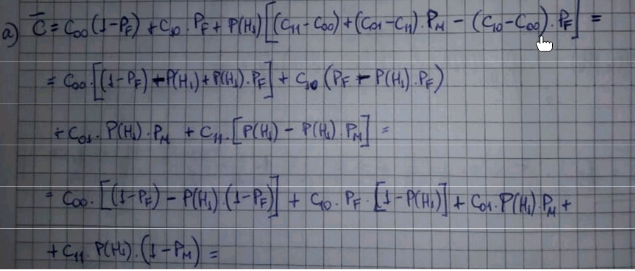
\includegraphics[width=0.6\textwidth]{./Imagenes/chinardo1.png}	
%\end{figure}

\begin{equation*}
	p(0) = \left[ \begin{array}{c} \vdots \\ 0 \\ 1 \\ 0 \\ \vdots \end{array} \right] \rightarrow P\left[ X(0) = 0 \right] = 1
\end{equation*}
\begin{equation*}
	P(1) = \begin{bmatrix}
				\hdots & 0 & 1/2 & 0 & 0 & 0 & \hdots & 0 \\
				\hdots & 1/2 & 0 & 1/2 & 0 & 0 & \hdots & 0 \\
				\hdots & 0 & 1/2 & 0 & 1/2 & 0 & \hdots & 0 \\
				\hdots & 0 & 0 & 1/2 & 0 & 1/2 & \hdots & 0 \\
				\hdots & 0 & 0 & 0 & 1/2 & 0 & \hdots & 0 \\
				\hdots & 0 & 0 & 0 & 0 & 1/2 & \hdots & 0 \\
				\hdots & \vdots & \vdots & \vdots & \vdots & \vdots & \hdots & 0 
		   \end{bmatrix}
\end{equation*}

\vspace{1cm}

\textbf{5.31}
\begin{equation*}
\begin{gathered}
	X(n+1) = X(n) - 1  \\
	P[U(n) = 0] = P[U(n) = 1] = P[U(n) = 2] = \frac{1}{3}
\end{gathered}
\end{equation*}

$X(n)$ es la cantidad de mensajes, mientras que $U(n)$ es la taza de arribos. Condición inicial: $X(0) = 1$ (En el instante 0 hay 1 mensaje), por lo tanto
\begin{equation*}
	p(0) = \left[ \begin{array}{c} 0 \\ 1 \\ 0 \\ 0 \\ \vdots \end{array} \right]
\end{equation*}

Sabiendo que tengo 1 mensaje en $t=1$ y $\frac{1}{3}$ de probabilidad de que llegue 0, 1 o 2 mensajes:
\begin{equation*}
	p(1) = \left[ \begin{array}{c} \textcolor{red}{1/3} \\ \textcolor{olive}{1/3} \\ \textcolor{blue}{1/3} \\ 0 \\ \vdots \end{array} \right]
\end{equation*}

De la misma forma:
\begin{equation*}
	p(1) = \left[ \begin{array}{c}
		\textcolor{red}{1/3 \ 1/3} + \textcolor{olive}{1/3 \ 1/3} + \textcolor{blue}{0} \\
		\textcolor{red}{1/3 \ 1/3} + \textcolor{olive}{1/3 \ 1/3} + \textcolor{blue}{1/3 \ 1/3} \\
		\textcolor{red}{1/3 \ 1/3} + \textcolor{olive}{1/3 \ 1/3} + \textcolor{blue}{1/3 \ 1/3} \\
		\textcolor{blue}{1/3 \ 1/3} \\
		0 \\ 0 \\ \vdots \end{array} \right]
\end{equation*}

Es decir, $p$ representa la probabilidad de tener $n$ mensajes en un t dado, con una condicion inicial fijada. Por otro lado, P representa la probabilidad de tener $n$ mensajes en un t dado para todas las condiciones iniciales.

\begin{equation*}
	P(1) = \begin{bmatrix}
				1/3 & 1/3 & 1/3 & 0 & 0 & 0 & \hdots \\
				1/3 & 1/3 & 1/3 & 0 & 0 & 0 & \hdots \\
				0 & 1/3 & 1/3 & 1/3 & 0 & 0 & \hdots \\
				0 & 0 & 1/3 & 1/3 & 1/3 & 0 & \hdots \\
				\vdots & \vdots & \vdots & \vdots & \vdots & \vdots & \hdots
		   \end{bmatrix}
\end{equation*}

\vspace{1cm}

\textbf{5.37} Ecuación 5.72:
%\begin{figure}[H]
%\centering
%	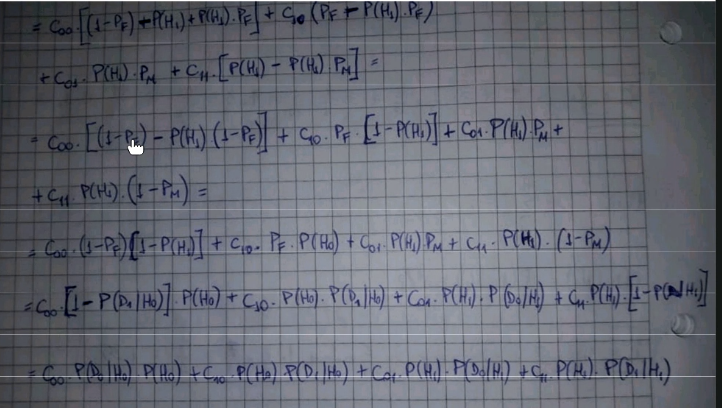
\includegraphics[width=0.6\textwidth]{./Imagenes/chinardo2.png}	
%\end{figure}

\begin{equation*}
\begin{split}
	\lim_{\epsilon \to 0} P_{k,j} (\epsilon) = \ & \lambda_{k,j} \epsilon	\	\ k \neq j	\\
	= \ & 1 + \lambda_{k,j} \epsilon 		\	\ k = j	
\end{split}
\end{equation*}

\begin{equation*}
\begin{split}
	P_{i,j} (\tau) = \ & \sum_{k} P_{i,k} (t) P_{k,j} (\tau - t) =  \underbrace{\sum_{k \neq j} P_{i,k} (t) \lambda_{kj} (\tau - t) + P_{i,j} \left[ 1 + \lambda_{kj} (\tau - t) \right]}_{\text{Usando la propiedad de este ejercicio}} \\
	= \ & \sum_{k \neq j} P_{i,k} (t) \lambda_{kj} (\tau - t) + P_{i,j} +  P_{i,j} \lambda_{kj} (\tau - t)	\\
	= \ & \sum_{k} P_{i,k} (t) \lambda_{k,j} (\tau - t) + P_{i,j}(t)
\end{split}
\end{equation*}

\vspace{0.5cm}

\begin{equation*}
\begin{gathered}
	P_{i,j} (\tau) = \sum_{k} P_{i,k} (t) \lambda_{k,j} (\tau - t) + P_{i,j}(t)	\\
	P_{i,j} (\tau) - P_{i,j}(t) = \sum_{k} P_{i,k} (t) \lambda_{k,j} (\tau - t) \\
	\frac{P_{i,j} (\tau) - P_{i,j}(t)}{\tau - t} = \sum_{k} P_{i,k} (t) \lambda_{k,j}
\end{gathered}
\end{equation*}

\vspace{1cm}

\textbf{5.38}
%\begin{figure}[H]
%\centering
%	\includegraphics[width=0.6\textwidth]{./Imagenes/chinardo3.png}	
%\end{figure}

\begin{equation*}
\begin{gathered}
	p_1(t) = \frac{\mu}{\lambda + \mu} + e^{-\left( \mu + \lambda \right) t} \cdot \frac{\lambda p_1 (0) - \mu p_2 (0)}{\lambda + \mu}	\\
	p_2(t) = 1 - p_1(t)
\end{gathered}
\end{equation*}

Con $p_1(0) = 0$ y $p_2(0) = 1$

\begin{equation*}
\begin{gathered}
	p_1(t) = -\frac{\mu}{\lambda + \mu} \left[ 1 + e^{-\left( \mu + \lambda \right) t} \right]	\\
	p_2(t) = \frac{\lambda}{\lambda + \mu} + \frac{\mu}{\lambda + \mu} e^{-\left( \mu + \lambda \right) t}
\end{gathered}
\end{equation*}

\begin{equation*}
\begin{gathered}
	\lim_{t \to \infty} p_1(t) = -\frac{\mu}{\lambda + \mu} \text{ y } \lim_{t \to \infty} p_2(t) = 1 - \frac{\mu}{\lambda + \mu} = \frac{\lambda}{\lambda + \mu}
\end{gathered}
\end{equation*}


\vspace{1cm}

\textbf{5.48} Se define $\lambda_a = \frac{5}{6} \frac{jobs}{min}$ y $\lambda_d = 1 \frac{jobs}{min}$, con $\rho = \frac{\lambda_a}{\lambda_d}$ y el Service Time $E \left\lbrace S \right\rbrace = \frac{1}{\lambda_d}$

a)
\begin{equation*}
\begin{split}
	E \left\lbrace W \right\rbrace = \frac{\rho}{1 - \rho}	E \left\lbrace S \right\rbrace = 5 \ min
\end{split}
\end{equation*}

b) $\lambda_d = 2 \frac{jobs}{min} \rightarrow E \left\lbrace W \right\rbrace = \frac{5}{14} $

c )$\lambda_a = \frac{5}{3} \frac{jobs}{min} \ \ \lambda_d = 2 \frac{jobs}{min} \rightarrow E \left\lbrace W \right\rbrace = 2.5 $

\vspace{1cm}

\textbf{5.54}


\newpage

\section*{CAP. VI}

\textbf{6.1}

\begin{equation*}
\begin{gathered}
	\mathcal{F}_{Y|H_0}(y|H_0) = 1 \ \ \ 0 \le1 y \leq 1	\\
	\mathcal{F}_{Y|H_1}(y|H_1) = 2y \ \ \ 0 \le1 y \leq 1
\end{gathered}
\end{equation*}

a)
\begin{equation*}
\begin{gathered}
	L(y) = \frac{2y}{1} \h \frac{1/2}{1/2}	\\
	y \overset{H_1}{\underset{H_0}{\gtrless}} \frac{1}{2}
\end{gathered}
\end{equation*}

b)
\begin{equation*}
\begin{split}
	P_e = P(H_0)P(D_1|H_0) + P(H_1)P(D_0|H_1) = \ & \frac{1}{2} \int_{1/2}^{1} f_{Y|H_0}(y|H_0) \ dy + \frac{1}{2} \int_{0}^{1/2} f_{Y|H_1}(y|H_1) \ dy \\
	 = \ & \frac{1}{2} \int_{1/2}^{1} 1 \ dy + \frac{1}{2} \int_{0}^{1/2} 2y \ dy = \frac{1}{4} + \frac{1}{8} = \frac{3}{8}
\end{split}
\end{equation*}

Si me hubiera dado mayor a $1/2$, me estaría delatando que está mal, no puedo tener una probabilidad mayor que a la del error.

\vspace{1cm}

\textbf{6.4}

\begin{figure}[H]
\centering
	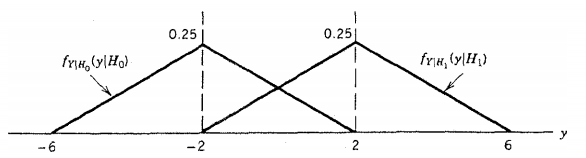
\includegraphics[width=0.6\textwidth]{Imagenes/enbessel1.png}
\end{figure}
\begin{equation*}
\begin{gathered}
	f_{Y|H_0}(y|H_0) = \frac{1}{4} \left( 1 - \left| \frac{x + 2}{4} \right| \right) \ \ \ -6 < y < 2 \\
	f_{Y|H_1}(y|H_1) = \frac{1}{4} \left( 1 - \left| \frac{x - 2}{4} \right| \right) \ \ \ -2 < y < 6
\end{gathered}
\end{equation*}


\begin{equation*}
\begin{gathered}
	\frac{f_{Y|H_1}(y|H_1)}{f_{Y|H_0}(y|H_0)} \h \frac{P(H_0) \left( C_{10} - C_{00} \right)}{P(H_1) \left( C_{01} - C_{11} \right)}
\end{gathered}
\end{equation*}

a)
Con $-2 \leq y \leq 2$:
\begin{equation*}
\begin{gathered}
	\frac{1/8 + y/16}{1/8 - y/16} \h \frac{1/3}{2/3}	\\
	y \h -\frac{2}{3}
\end{gathered}
\end{equation*}

Costo medio (\textbf{formula}):
\begin{equation*}
\begin{gathered}
	\overline{C} = C_{00} P(H_0) P(D_0|H_0) + C_{01} P(H_1) P(D_0|H_1) + C_{10} P(H_0) P(D_1|H_0) + C_{11} P(H_1) P(D_1|H_1)
\end{gathered}
\end{equation*}

\begin{equation*}
\begin{gathered}
	\overline{C} = 1 \cdot \frac{1}{3} \cdot \frac{7}{9} + 3 \cdot \frac{2}{3} \cdot \frac{1}{18} + 3 \cdot \frac{1}{3} \cdot \frac{2}{9} + 1 \cdot \frac{2}{3} \cdot \frac{17}{18} = \frac{11}{9} \approx 1.2222
\end{gathered}
\end{equation*}

b)

\begin{equation*}
\begin{gathered}
	\overline{C} = 1 \cdot \frac{1}{3} \cdot \frac{7}{8} + 3 \cdot \frac{2}{3} \cdot \frac{1}{8} + 3 \cdot \frac{1}{3} \cdot \frac{1}{8} + 1 \cdot \frac{2}{3} \cdot \frac{7}{8} = \frac{5}{4} = 1.25
\end{gathered}
\end{equation*}

\vspace{1cm}

\textbf{6.7}

a)

\begin{equation*}
\begin{gathered}
	P_F = P(D_1|H_0)	\\
	P_M = P(D_0|H_1)
\end{gathered}
\end{equation*}

%\begin{equation*}
%\begin{split}
%	\bar{C} = \ & C_{00} (1 - P_F) + C_{10} P_F + P(H_1) \left[\left( C_{11} - C_{00} \right) + \left( C_{01} - C_{11} \right) P_M - \left( C_{10} - C_{00} \right) P_F \right] \\
%	= \ & C_{00} P(D_0|H_0) + C_{10} P(D_1|H_0) + P(H_1) \left[\left( C_{11} - C_{00} \right) + \left( C_{01} - C_{11} \right) P(D_0|H_1) - \left( C_{10} - C_{00} \right) P(D_1|H_0) \right] \\
%	= \ & C_{00} \left[ P(D_0|H_0) - P(H_1) + P(H_1) P(D_1|H_0) \right] + C_{01} \left[ P(H_1) P(D_0|H_1) + P(H_1) \right] + \\ & + C_{10} \left[ P(D_1|H_0) - P(H_1) P(D_1|H_0) \right]  + C_{1} \left[ P(H_1) - P(H_1) P(D_0|H_1) \right] 
%\end{split}
%\end{equation*}

\begin{figure}[H]
\centering
	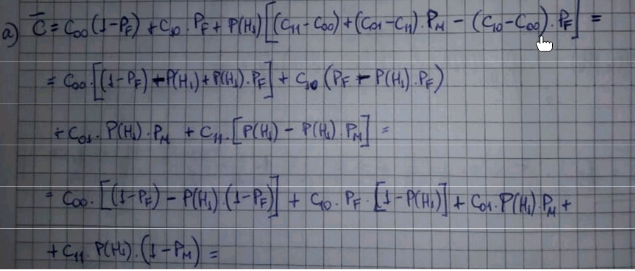
\includegraphics[width=1\textwidth]{Imagenes/chinardo1.png}
\end{figure}

\begin{figure}[H]
\centering
	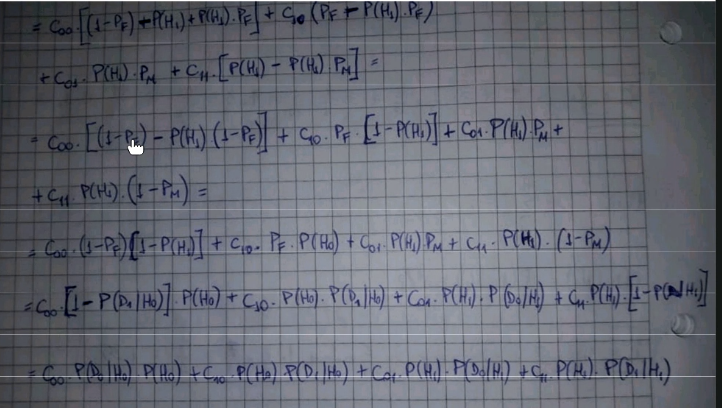
\includegraphics[width=1\textwidth]{Imagenes/chinardo2.png}
\end{figure}

b)

\vspace{1cm}

\textbf{6.13}
\begin{equation*}
\begin{gathered}
	f_{Y|H_0}(y|H_0) = \frac{1}{2} e^{-y/2} \ \ \ 0 < y \\
	f_{Y|H_1}(y|H_1) = \frac{1}{4} e^{-y/4} \ \ \ 0 < y
\end{gathered}
\end{equation*}

a)
\begin{equation*}
\begin{gathered}
	\frac{f_{Y_1, Y_2 |H_1}(y_1, y_2|H_1)}{f_{Y_1, Y_2 |H_0}(y_1, y_2|H_0)} = \frac{\frac{1}{16} e^{-(y_1/4) - (y_2/4)}}{\frac{1}{4} e^{-(y_1/2) - (y_2/2)}} \h 1	\\
	e^{(y_1/4) + (y_2/4)} \h 4 \\
	y_1 + y_2 \h 4 \ Ln(4)
\end{gathered}
\end{equation*}

b)
\begin{equation*}
\begin{split}
	P_M = P(D_0|H_1) = \ & \int_{0}^{4Ln(4)} \int_{0}^{4Ln(4) - y_2} f_{Y_1, Y_2 |H_1}(y_1, y_2|H_1) dy_1 dy_2 \\
	= \ & \int_{0}^{4Ln(4)}  \frac{e^{-y_2/4}}{4} \frac{4 - e^{y_2/4}}{4} dy_2 = -\frac{\ Ln(4) - 3}{4} \approx 0.4034
\end{split}
\end{equation*}

\begin{equation*}
\begin{split}
	P_F = P(D_1|H_0) = \ & \int_{0}^{4Ln(4)} \int_{4Ln(4) - y_1}^{\infty} f_{Y_1, Y_2 |H_0}(y_1, y_2|H_0) dy_2 dy_1 + \int_{4Ln(4)}^{\infty} \int_{0}^{\infty} f_{Y_1, Y_2 |H_0}(y_1, y_2|H_0) dy_2 dy_1 \\
	= \ & \int_{0}^{4Ln(4)} \frac{e^{-y_1/2}}{2} \frac{e^{-y_1/2}}{16} dy_1 + \int_{4Ln(4)}^{\infty} \frac{e^{-y_1/2}}{2} dy_1 = \frac{255}{8192} + \frac{1}{16} \approx 0.0936
\end{split}
\end{equation*}

\newpage

\section*{CAP. VII}

\textbf{7.7}

Pag. 387.

\begin{equation*}
	\begin{bmatrix}
		R_{SS}(0) & R_{SS}(1) & R_{SS}(2) \\
		R_{SS}(1) & R_{SS}(0) & R_{SS}(1) \\
		R_{SS}(2) & R_{SS}(1) & R_{SS}(0) 
	\end{bmatrix}
	\cdot
	\begin{bmatrix}
		h_1 \\
		h_2 \\
		h_3 
	\end{bmatrix}
	=
	\begin{bmatrix}
		R_{SS}(1) \\
		R_{SS}(2) \\
		R_{SS}(3) 
	\end{bmatrix}
\end{equation*}	
\begin{equation*}
	\begin{bmatrix}
		1 & 0.9 & 0.7 \\
		0.9 & 1 & 0.9 \\
		0.7 & 0.9 & 1 
	\end{bmatrix}
	\cdot
	\begin{bmatrix}
		h_1 \\
		h_2 \\
		h_3 
	\end{bmatrix}
	=
	\begin{bmatrix}
		0.9 \\
		0.7 \\
		0.6
	\end{bmatrix}	
\end{equation*}
\begin{equation*}
\begin{bmatrix}
		h_1 \\
		h_2 \\
		h_3 
	\end{bmatrix}
	=
	\begin{bmatrix}
		2 \\
		-2 \\
		1
	\end{bmatrix}	
\end{equation*}

\begin{equation*}
\begin{gathered}
	\hat{S}(n) = h_1 S(n-1) + h_2 S(n-2) + h_3 S(n-3) 
\end{gathered}
\end{equation*}

\vspace{1cm}

\textbf{7.14}
\begin{equation*}
\Sigma_{XX} = 
	\begin{bmatrix}
		2 & 1 & 1/2 \\
		1 & 3 & 1 \\
		1/2 & 1 & 4 
	\end{bmatrix}
\end{equation*}

Se sabe que:
\begin{equation*}
\begin{gathered}
	\gamma (n,n) = 1
\end{gathered}
\end{equation*}

\begin{equation*}
	\begin{bmatrix}
		1 & 0 & 0 \\
		\gamma(2,1) & 1 & 0 \\
		\gamma(3,1) & \gamma(3,2) & 1
	\end{bmatrix}
	\cdot
	\begin{bmatrix}
		X(1) \\
		X(2) \\
		X(3) 
	\end{bmatrix}
	=
	\begin{bmatrix}
		V_X(1) \\
		V_X(2) \\
		V_X(3) 
	\end{bmatrix}
\end{equation*}	

Como la media es nula
\begin{equation*}
\begin{gathered}
	C_{XX}(t_1, t_2) = R_{XX}(t_1, t_2) - \mu_{X}(t_1) \mu_{X}(t_2) = R_{XX}(t_1, t_2)
\end{gathered}
\end{equation*}

Eq. 7.70:
\begin{equation*}
\begin{gathered}
	\gamma (2,1) = -\frac{R_{XX}(1,2)}{R_{XX}(1,1)} = -\frac{1}{2}
\end{gathered}
\end{equation*}

Las \textbf{innovaciones} son ortogonales, por lo tanto:
\begin{equation*}
\begin{gathered}
	E\left\lbrace V_X(1) V_X(3) \right\rbrace = 0 \\
	E\left\lbrace X(1) \left[ \gamma(3,1)X(1) + \gamma(3,2)X(2) + X(3)\right] \right\rbrace = 0 \\	
	\gamma(3,1)R_{XX}(1,1) + \gamma(3,2)R_{XX}(1,2) + R_{XX}(1,3) = 0	\\
	2\gamma(3,1) + \gamma(3,2) + \frac{1}{2} = 0
\end{gathered}
\end{equation*}

\begin{equation*}
\begin{gathered}
	E\left\lbrace V_X(2) V_X(3) \right\rbrace = 0 \\
	E\left\lbrace \left[ X(1) \gamma(2,1) + X(2) \right] \left[ \gamma(3,1)X(1) + \gamma(3,2)X(2) + X(3)\right] \right\rbrace = 0 \\
	-\gamma(3,1) - \frac{\gamma(3,2)}{2} - \frac{1}{4} + \gamma(3,1) + 3 \gamma(3,2) + 1  = 0 \\
	\gamma(3,2) = - \frac{3}{4} \cdot \frac{2}{5} = -\frac{3}{10}
\end{gathered}
\end{equation*}

\begin{equation*}
\begin{gathered}
	\gamma(3,1) = -\frac{1}{10}
\end{gathered}
\end{equation*}

\begin{equation*}
	\Gamma = \begin{bmatrix}
		1 & 0 & 0 \\
		-0.5 & 1 & 0 \\
		-0.1 & -0.3 & 1
	\end{bmatrix}
	\Longrightarrow \mathbb{L} = \Gamma^{-1} =
	\begin{bmatrix}
		1 & 0 & 0 \\
		0.5 & 1 & 0 \\
		0.25 & 0.3 & 1
	\end{bmatrix}
\end{equation*}	

\end{document}